% ----------------------------------------------------
% Literature Review
% ----------------------------------------------------
%\documentclass[class=report,11pt,crop=false]{standalone}
%% Page geometry
\usepackage[a4paper,margin=20mm,top=25mm,bottom=25mm]{geometry}

% Font choice
\usepackage{lmodern}

% Use IEEE bibliography style
\bibliographystyle{IEEEtran}

% Line spacing
\usepackage{setspace}
\setstretch{1.20}

% Allows us to create dummy text
\usepackage{lipsum}

% Ensure UTF8 encoding
\usepackage[utf8]{inputenc}

% Language standard (not too important)
\usepackage[english]{babel}

% Skip a line in between paragraphs
\usepackage{parskip}

% For the creation of dummy text
\usepackage{blindtext}

% Math
\usepackage{amsmath}

% Header & Footer stuff
\usepackage{fancyhdr}
\pagestyle{fancy}
\fancyhead{}
\fancyhead[R]{\nouppercase{\rightmark}}
\fancyfoot{}
\fancyfoot[C]{\thepage}
\renewcommand{\headrulewidth}{0.0pt}
\renewcommand{\footrulewidth}{0.0pt}
\setlength{\headheight}{13.6pt}

% Epigraphs
\usepackage{epigraph}
\setlength\epigraphrule{0pt}
\setlength{\epigraphwidth}{0.65\textwidth}

% Colour
\usepackage{color}
\usepackage[dvipsnames]{xcolor}

% Hyperlinks & References
\usepackage{hyperref}
\definecolor{linkColour}{RGB}{77,71,179}
\hypersetup{
    colorlinks=true,
    linkcolor=linkColour,
    filecolor=linkColour,
    urlcolor=linkColour,
    citecolor=linkColour,
}
\urlstyle{same}

% Automatically correct front-side quotes
\usepackage[autostyle=false, style=ukenglish]{csquotes}
\MakeOuterQuote{"}

% Graphics
\usepackage{graphicx}
\graphicspath{{Images/}{../Images/}}
\usepackage{makecell}
\usepackage{transparent}

% SI units
\usepackage{siunitx}

% Microtype goodness
\usepackage{microtype}

% Listings
\usepackage[T1]{fontenc}
\usepackage{listings}
\usepackage[scaled=0.8]{DejaVuSansMono}

% Custom colours for listings
\definecolor{backgroundColour}{RGB}{250,250,250}
\definecolor{commentColour}{RGB}{73, 175, 102}
\definecolor{identifierColour}{RGB}{196, 19, 66}
\definecolor{stringColour}{RGB}{252, 156, 30}
\definecolor{keywordColour}{RGB}{50, 38, 224}
\definecolor{lineNumbersColour}{RGB}{127,127,127}
\lstset{
  language=Matlab,
  captionpos=b,
  aboveskip=15pt,belowskip=10pt,
  backgroundcolor=\color{backgroundColour},
  basicstyle=\ttfamily,%\footnotesize,        % the size of the fonts that are used for the code
  breakatwhitespace=false,         % sets if automatic breaks should only happen at whitespace
  breaklines=true,                 % sets automatic line breaking
  postbreak=\mbox{\textcolor{red}{$\hookrightarrow$}\space},
  commentstyle=\color{commentColour},    % comment style
  identifierstyle=\color{identifierColour},
  stringstyle=\color{stringColour},
   keywordstyle=\color{keywordColour},       % keyword style
  %escapeinside={\%*}{*)},          % if you want to add LaTeX within your code
  extendedchars=true,              % lets you use non-ASCII characters; for 8-bits encodings only, does not work with UTF-8
  frame=single,	                   % adds a frame around the code
  keepspaces=true,                 % keeps spaces in text, useful for keeping indentation of code (possibly needs columns=flexible)
  morekeywords={*,...},            % if you want to add more keywords to the set
  numbers=left,                    % where to put the line-numbers; possible values are (none, left, right)
  numbersep=5pt,                   % how far the line-numbers are from the code
  numberstyle=\tiny\color{lineNumbersColour}, % the style that is used for the line-numbers
  rulecolor=\color{black},         % if not set, the frame-color may be changed on line-breaks within not-black text (e.g. comments (green here))
  showspaces=false,                % show spaces everywhere adding particular underscores; it overrides 'showstringspaces'
  showstringspaces=false,          % underline spaces within strings only
  showtabs=false,                  % show tabs within strings adding particular underscores
  stepnumber=1,                    % the step between two line-numbers. If it's 1, each line will be numbered
  tabsize=2,	                   % sets default tabsize to 2 spaces
  %title=\lstname                   % show the filename of files included with \lstinputlisting; also try caption instead of title
}

% Caption stuff
\usepackage[hypcap=true, justification=centering]{caption}
\usepackage{subcaption}

% Glossary package
% \usepackage[acronym]{glossaries}
\usepackage{glossaries-extra}
\setabbreviationstyle[acronym]{long-short}

% For Proofs & Theorems
\usepackage{amsthm}

% Maths symbols
\usepackage{amssymb}
\usepackage{mathrsfs}
\usepackage{mathtools}

% For algorithms
\usepackage[]{algorithm2e}

% Spacing stuff
\setlength{\abovecaptionskip}{5pt plus 3pt minus 2pt}
\setlength{\belowcaptionskip}{5pt plus 3pt minus 2pt}
\setlength{\textfloatsep}{10pt plus 3pt minus 2pt}
\setlength{\intextsep}{15pt plus 3pt minus 2pt}

% For aligning footnotes at bottom of page, instead of hugging text
\usepackage[bottom]{footmisc}

% Add LoF, Bib, etc. to ToC
\usepackage[nottoc]{tocbibind}

% SI
\usepackage{siunitx}

% For removing some whitespace in Chapter headings etc
\usepackage{etoolbox}
\makeatletter
\patchcmd{\@makechapterhead}{\vspace*{50\p@}}{\vspace*{-10pt}}{}{}%
\patchcmd{\@makeschapterhead}{\vspace*{50\p@}}{\vspace*{-10pt}}{}{}%
\makeatother
%
\newacronym{radar}{RADAR}{Radio Detection and Ranging}

%\begin{document}
\ifstandalone
\tableofcontents
\fi
% ----------------------------------------------------
\chapter{Literature Review \label{ch:literature}}
%\epigraph{If you wish to make an apple pie from scratch, you must first invent the universe.}%
%    {\emph{---Carl Sagan}}
%\vspace{0.5cm}
% ----------------------------------------------------
\section{Antenna}\label{sec:antenna}
\subsection{Antenna Gain}
An antenna is a RF device that transfers energy from closed system to free space. Antennas are usually designed to be pointed at an object, receiver, or scene. Therefor an antenna is designed to have the majority of its power radiated in the direction it’s facing. This is known as the directivity of an antenna. The antenna pattern provides a visual representation of an antenna’s directivity as seen in figure \ref{fig:chp2_antenna_pattern}. The antenna main lobe includes the energy radiated in the intended direction, whereas the back lobe and side lobes include energy radiated in all other directions. The higher the side lobes, the less energy is radiated in the main lobe. Side lobes are an unavoidable byproduct of antenna design, however there are techniques to decrease the SLL (Side Lobe Level). The Antenna Gain is measured in either dBi or dBd which is the decibel level relative to a isotropic radiator or dipole respectively.

    \begin{figure}[H]
    \centering
    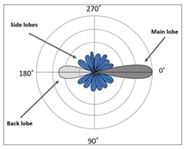
\includegraphics[width=0.3\linewidth]{Figures/chp2_antenna_pattern.png}
    \caption{A typical Antenna pattern.}
    \label{fig:chp2_antenna_pattern}
    \end{figure}

\subsection{Nearfield \& Farfield}
As seen in the figure \ref{fig:chp2_planarwave}, the greater the distance away from the antenna more planar the transmitted waves become. The region where the transmitted wave can safely be approximated as a planar wave is known as the Far field. The Region between the antenna and the far field is known as the nearfield region and in general radars operate in the Farfield. The Farfield distance depends on the maximum dimension of the antenna’s radiating surface or aperture, \cite{Farfield}.

    \begin{figure}[H]
    \centering
    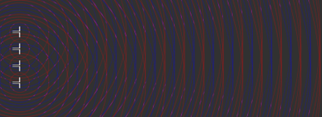
\includegraphics[width=0.6\linewidth]{Figures/chp2_planarwave.png}
    \caption{Transition from spherical waves to planar waves.}
    \label{fig:chp2_planarwave}
    \end{figure}

According to \cite{Farfield} the distance is depended on the maximum dimension of the antenna and is calculated as
    \[R_{ff}=\frac{2D^{2}}{\lambda}\]

Most antennas are resonant structures or at the very least consist out of multiple resonant structures, meaning that they have narrow bandwidths due to some dimension of the antenna being a fraction of the signal wavelength at the center frequency (\(f_{0}\)).

\subsection{Monopole Antenna}
One such resonant antenna is the monopole antenna. It can be built by simply cutting a cable to the resonant length, which is a quarter of a wavelength at the center frequency. A monopole does not have high directivity as it has an omnidirectional radiation pattern in azimuth, see figure below. Other forms of antennas are more complicated to design and manufacture, but they offer better directivity, allowing the operator to focus more of the energy in the direction of interest. Typical monopole antennas have a gain of 2-5 dBi.

    \begin{figure}[H]
    \centering
    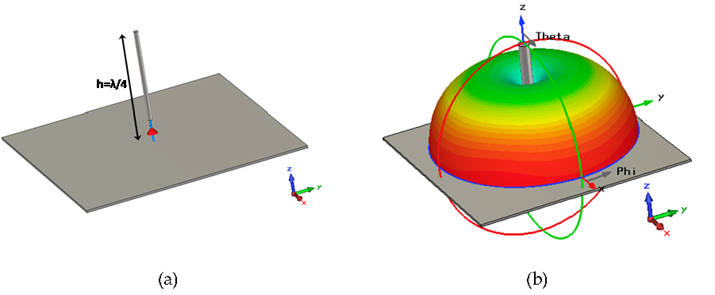
\includegraphics[width=0.6\linewidth]{Figures/chp2_monopole.png}
    \caption{Monopole model and 3D antenna pattern.}
    \label{fig:chp2_monopole}
    \end{figure}

\subsection{Patch Antenna}
An example of an antenna with higher directivity is a patch antenna. A patch can be designed to have gain raging between 5-10 dBi. The patch antenna is still a resonant antenna as it has narrow bandwidths and the center frequency is determined by the length of the (L) and the substrate used, see figure \ref{fig:chp2_patch}. Equations see below from \cite{patchDimensions}

    \begin{figure}[H]
    \centering
    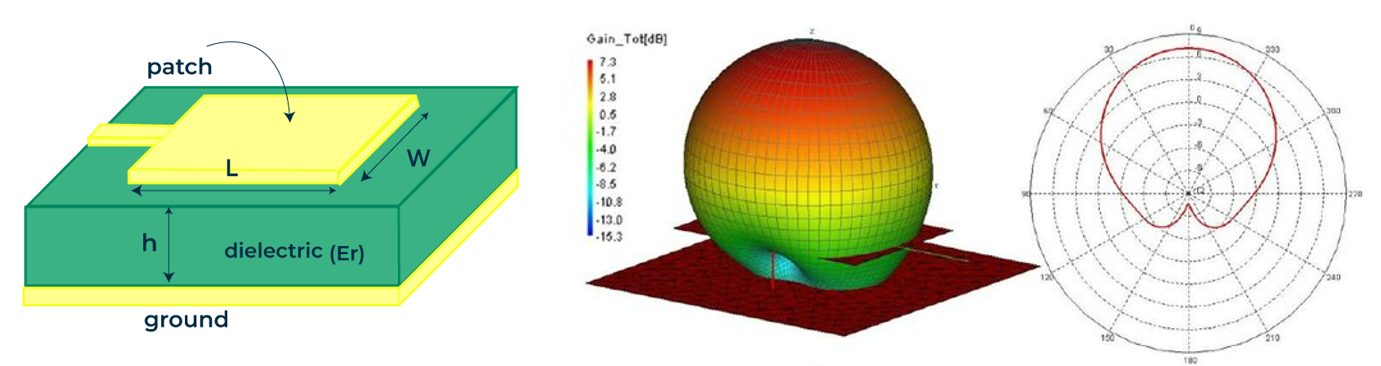
\includegraphics[width=0.8\linewidth]{Figures/chp2_patch.png}
    \caption{Patch antenna model and antenna pattern.}
    \label{fig:chp2_patch}
    \end{figure}

For the design equations of a patch antenna it is assumed that the thickness of the substrate is significantly smaller than a wavelength at the center frequency of the antenna. The equation becomes inaccurate if this assumption does not hold due to fringing fields, see figure \ref{fig:chp2_fringing_fields}. The fringing fields increase the effective length of the antenna, in turn lowering the center frequency \cite{Fringing}.

    \begin{figure}[H]
    \centering
    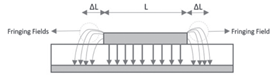
\includegraphics[width=0.5\linewidth]{Figures/chp2_fringing_fields.png}
    \caption{Fringing fields on a patch antenna.}
    \label{fig:chp2_fringing_fields}
    \end{figure}

The bandwidth of the antenna is determined by the width of the patch and can be calculated with the equation below.
    \[B=3.77\frac{\epsilon_{r}-1}{\epsilon_{r}^{2}}\frac{W}{L}\frac{t}{\lambda}\]

Since RF circuits are designed for a certain characteristic impedance and the edge of a patch is usually at a different impedance, the impedance must be transformed. The impedance at the edge of the patch is given by
    \[Z_{A}=90\frac{\epsilon_{r}^{2}}{\epsilon_{r}-1}\left( \frac{L}{W} \right)^{2}\]

As the antenna feed point is moved from the edge of the patch to the center of the patch, the impedance decreases until it reaches 0$\Omega$ at the middle of the patch.
    \[Z_{A}\left( \Delta x_{p} \right)=Z_{A}\left( \Delta x_{p}=0 \right)cos^{2}\left( \frac{\pi\Delta x_{p}}{L} \right)\]

\subsection{Horn Antenna}
For applications where more gain is needed, aperture antennas are commonly used. One such aperture antenna is the Horn antenna as they typically have more than 15dBi of gain. The advantage of the horn antenna is the high gain and high bandwidth. The disadvantage of the horn antenna is larger physical size of the antenna.

    \begin{figure}[H]
    \centering
    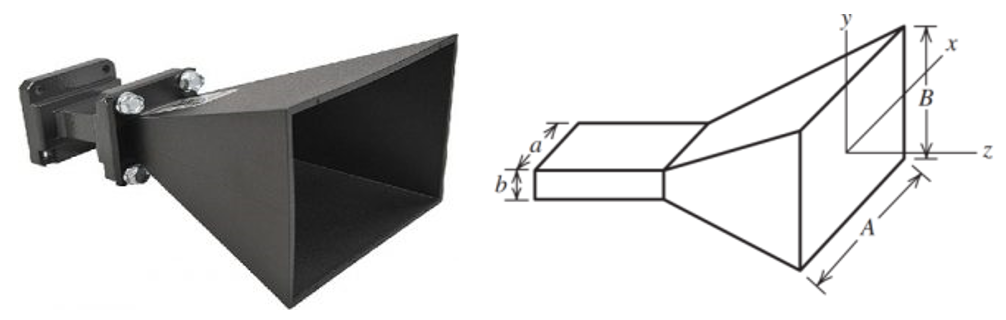
\includegraphics[width=0.6\linewidth]{Figures/chp2_Horn.png}
    \caption{A typical horn antenna.}
    \label{fig:chp2_Horn}
    \end{figure}

The gain of a pyramidal horn can be calculated as, assuming an aperture efficiency of 50\%, \cite{Horn}
    \[G=0.5\left( \frac{4\pi}{\lambda^{2}}AB \right)\]

\section{Radar Range Equation}
The maximum range of a radar system depends on the transmitted power (Pt), the received power (Pr), the transmitter antenna gain (Gt), the receiver antenna gain (Gr), the wavelength ($\lambda$) and the radar cross section ($\sigma$), \cite{Farfield}. The wavelength is proportional to the transmitted wave’s frequency. The radar cross section refers to the area visible from the transmitter. 
    \[P_{r}=\frac{P_{t}G^{2}\lambda^{2}\sigma}{\left( 4\pi \right)^{3}R^{4}}\]

\section{Frequency bands}
As the Electromagnetic (EM) spectrum is a limited resource it is divided up into different frequency bands for different wireless transmission applications. Radars tend to operate between  chose the operating frequency based on the range and resolution of the planned 1-40GHz. Since the wavelength inversely proportional to the frequency, the higher the frequency the physically smaller Radar and RF equipment become. Producing accurate but smaller radars becomes more expensive due to the component cost as well as the RF test equipment needed for the development.

    \begin{figure}[H]
    \centering
    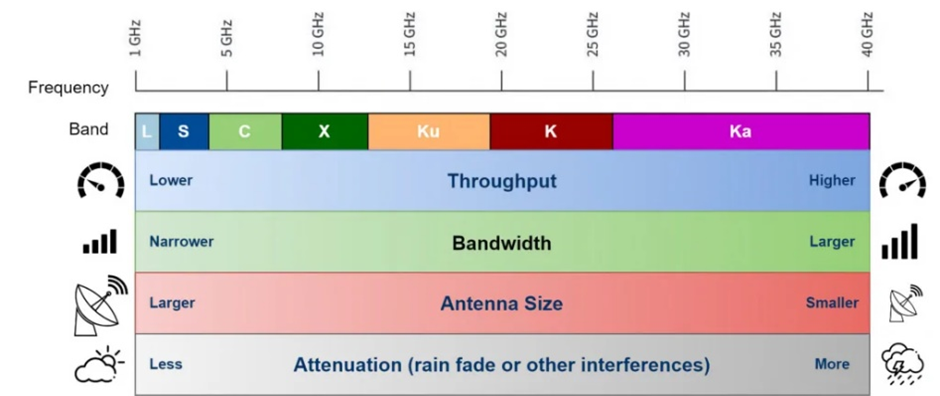
\includegraphics[width=0.8\linewidth]{Figures/chp2_EM_spectrum.png}
    \caption{Assigned Frequency Band in the EM spectrum.}
    \label{fig:chp2_EM_spectrum}
    \end{figure}
    
\section{\texorpdfstring{RF system impedance (50 $\Omega$ matched systems)}{The Omega Symbol}}\label{sec:OCSO50}
Impedance matching is a fundamental aspect of RF design and testing; the signal reflections caused by a mismatched impedance can lead to unwanted behavior and losses. The standardized RF impedance is 50$\Omega$, but it is important to understand that any other impedance can be used, but most COTS RF components are designed for 50$\Omega$ systems, \cite{50Ohm}.

In a closed 50$\Omega$ system between each of the components the quality of the match (how close to 50$\Omega$ to component is) is characterized by an input Return Loss ($RL_{in}$) and an output Return Loss ($RL_{out}$). The worse the match the more power is reflected back in the opposite direction of propagation, i.e. power lost. The worst RL possible is either an open circuit ($\infty$$\Omega$) or a short circuit (0$\Omega$). Both and open and short circuit reflects all the power, however a short circuit reflects the signal with a change in phase of 180°. An open circuit reflects the signal without a change in phase, see figure \ref{fig:chp2_sinwave_reflection}, \cite{VSWR}.

    \begin{figure}[H]
    \centering
    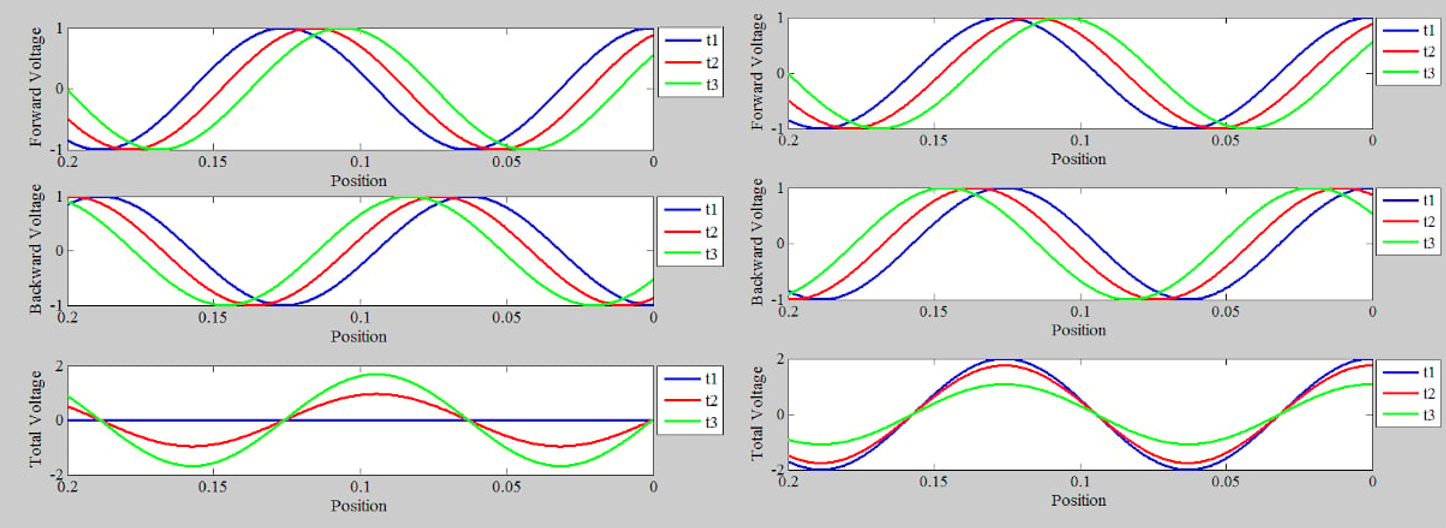
\includegraphics[width=0.9\linewidth]{Figures/chp2_sinwave_reflection.png}
    \caption{Reflection of a sinusoidal wave at an open circuit (left) and short circuit (right).}
    \label{fig:chp2_sinwave_reflection}
    \end{figure}

\subsection{Smith Chart}
The smith chart is a useful tool for RF design. It provides a visual method to characterize the impedance of RF components and transmission lines. A short perfect 0$\Omega$ would be plotted on the far left of the, a perfect 50$\Omega$ would be plotted at the origin and a perfect open circuit would be plotted on the far right of the smith chart.  The smith chart also allows the designer to determine what type of impedance transformation is needed as seen in the figure \ref{fig:chp2_smithchart}.

    \begin{figure}[H]
    \centering
    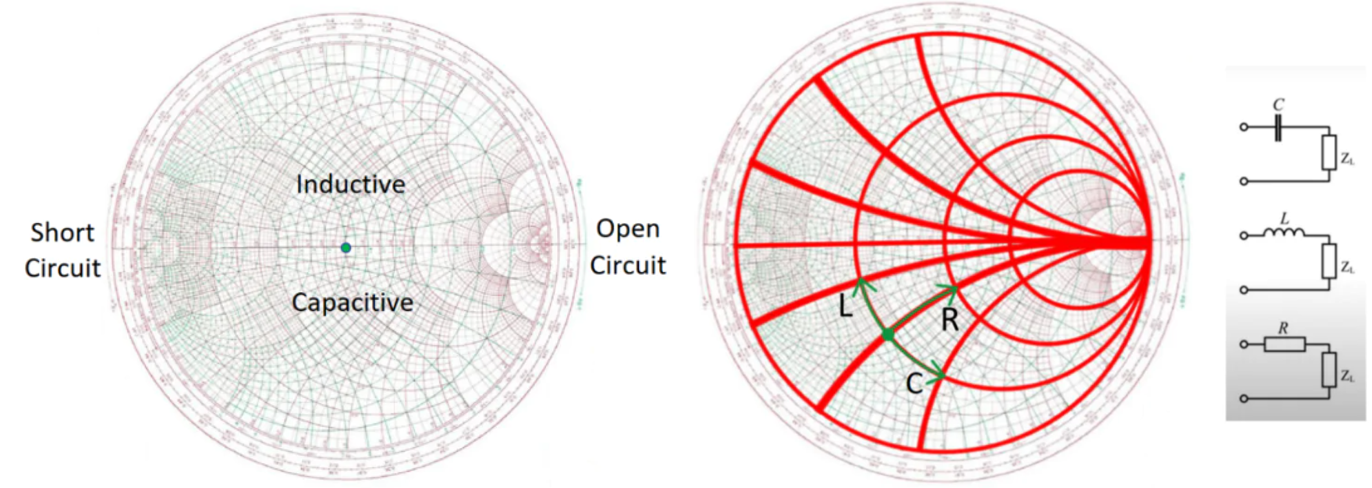
\includegraphics[width=0.8\linewidth]{Figures/chp2_smithchart.png}
    \caption{Smith chart and how lumped element move on the smith chart.}
    \label{fig:chp2_smithchart}
    \end{figure}

\section{Dielectric materials}
Printed Circuit Boards (PCB) consist of multiple electrically conductive layers. The substrate separates these electrically conductive layers is known as a dielectric. Multiple dielectric types exist and choosing the dielectric effects the entire RF design. The width for a 50$\Omega$ trace on a PCB depends on the type of dielectric as well as the thickness of the chosen substrate.

FR4 is the most common dielectric, but it is very lossy when used at high frequencies \cite{FR4}. High frequency PCB uses more expensive dielectric materials such as Rogers RO4003C, which have mush lower losses at high frequencies, but cost 10 times more .

In free space a signal propagates at the speed of light (\(c_{0}\)), however in a dielectric medium the velocity of propagation is decreased by a factor of \(\frac{1}{\sqrt{\epsilon_{r}}}\) . The effect is also observed with the wavelength decreasing in the dielectric and can be mathematically described below, \cite{Wavelength}.
    \[\lambda=\frac{c}{f\sqrt{\epsilon_{r}}}\]

\subsection{PCB Transmission lines}
Many different types of transmission lines can be designed for RF trace on and within a PCB. The most common is microstrip and its impedance can be calculated as 

    \begin{figure}[H]
    \centering
    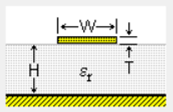
\includegraphics[width=0.25\linewidth]{Figures/chp2_microstrip.png}
    \caption{Microstrip model.}
    \label{fig:chp2_microstrip}
    \end{figure}
    \[Z_{0}=\frac{87}{\sqrt{\epsilon_{r}+1.41}}ln\left( \frac{5.98H}{0.8W+T} \right)\]

Other common types include Stripline, Coplanar Waveguide (CPW) and Coplanar Waveguide with ground (GCPW). A visual representation of all there can be seen in figure below. Each transmission line type becomes more elaborate to calculate the impedance of the trace, fortunately the dielectric manufacturers tend to provide calculator tools to calculate the impedance.

    \begin{figure}[H]
    \centering
    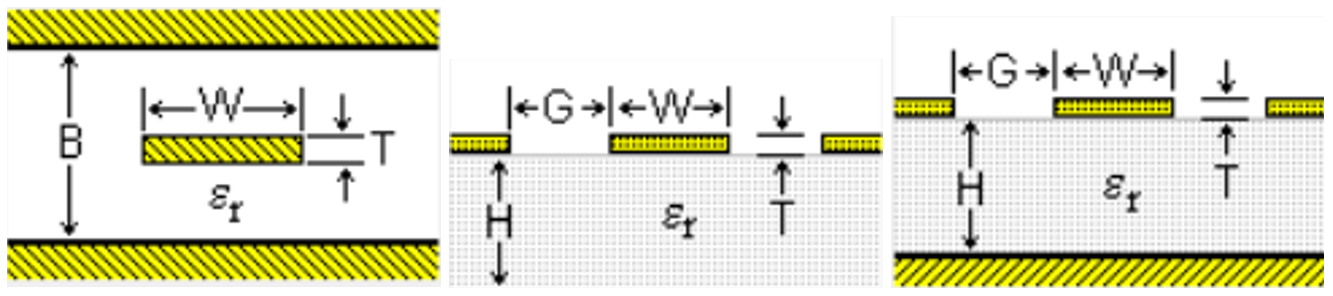
\includegraphics[width=0.65\linewidth]{Figures/chp2_transmission_lines.png}
    \caption{Stripline model (left), CPW model (middle) and GCPW model (right).}
    \label{fig:chp2_transmission_lines}
    \end{figure}

\subsection{Coaxial Cables}
Another type of RF transmission line that is commonly used for RF cables is the round Coaxial transmission line. These coaxial cables are ussually sold as 50$\Omega$ or 75$\Omega$ cables.

    \begin{figure}[H]
    \centering
    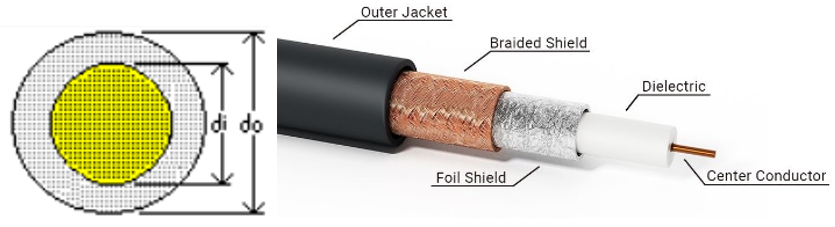
\includegraphics[width=0.7\linewidth]{Figures/chp2_coaxial_cable.png}
    \caption{Coaxial Cable.}
    \label{fig:chp2_coaxial_cable}
    \end{figure}

\section{FMCW}

    \begin{figure}[H]
    \centering
    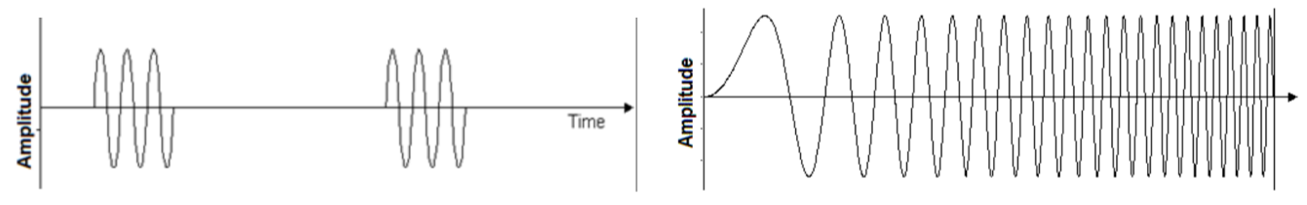
\includegraphics[width=1\linewidth]{Figures/chp2_FMCW.png}
    \caption{Pulsed waveform (left), FMCW waveform (right).}
    \label{fig:chp2_FMCW}
    \end{figure}
    
Two main types of radars exist, pulsed radars and continuous wave radars. A pulsed radar transmits a pulse and waits for the reflected pulse. Since the radar only transmits for a short period, the radar can transmit a high-powered pulse. This ensures a large maximum range for the radar. The duty cycle of the radar refers to the ratio of transmit time to the total time. Usually, the larger the transmitted power is, the shorter the pulse will be. This is to reduce the total power draw during operations. Unfortunately, the radar is blind while waiting for the returned pulse \cite{FMCW}. A pulsed radar usually operates at a single frequency lower than 50kHz. A Frequency Modulated Continuous Wave (FMCW) radar transmits continuously, and therefore at lower power than a pulse radar. The maximum range is thus also lower, but the radar is never blind. The waves frequency is varied when transmitting, this is done to differentiate the received signal and determine the propagation delay \cite{FMCW}. The frequency sweep of a FMCW radar can either be sweep up or sweep down with a large frequency range, typically from 1GHz to 40GHz.

\section{RF simulation software}
To complex RF components \& antennas becomes a computationally intensive exercise. Many software suites are available to solve the EM performance of a designed 3D model. To two software suites available at the time of this report were Altair FEKO and Dassault Systèmes CST Studio Suite.

\subsection{FEKO}
FEKO is commonly used for antenna design, the Farfield performance of a designed structure as well as EMC compliance. FEKO is easy to understand with a minimal learning curve when designing antennas, however its UI is still limited at the time of the report. The minimum mesh size is much larger than CST Studio, however there are methods to force a smaller mesh at certain places by adding a second slightly smaller copper block over an existing copper block. FEKO’s parameter sweep macro runs on a CMD window and creates a separate CAD model for each parameter change which is solved individually. The results cannot be viewed together, unless the entire parameter sweep has run successfully and the .xml file was automatically generated.

    \begin{figure}[H]
    \centering
    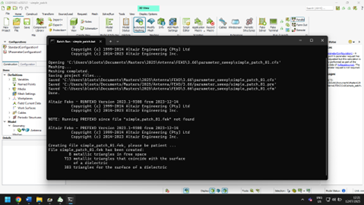
\includegraphics[width=0.9\linewidth]{Figures/chp2_FEKO_parameter_sweep.png}
    \caption{Running a parameter sweep in FEKO.}
    \label{fig:chp2_FEKO_parameter_sweep}
    \end{figure}

FEKO also provides more port options and source options. An edge port is very simple to implement for a microstrip line, but not for a CPW line. The help documentation is quite limited.

    \begin{figure}[H]
    \centering
    
\includegraphics[width=0.95\linewidth]{Figures/chp2_FEKO_ports.png}
    \caption{Available ports and sources in FEKO.}
    \label{fig:chp2_FEKO_ports}
    \end{figure}

\subsection{CST}
CST Studio on the other hand has a steeper learning curve, but a much more extensive UI and help documentation. CST Studio only uses two port types, but the waveguide port can be used for most feeds including microstrip, stripline and CPW. CST also provides a macro that constructs the port correctly on the picked face.

    \begin{figure}[H]
    \centering
    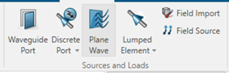
\includegraphics[width=0.4\linewidth]{Figures/chp2_CST_ports.png}
    \caption{Available ports and sources in CST.}
    \label{fig:chp2_CST_ports}
    \end{figure}

    \begin{figure}[H]
    \centering
    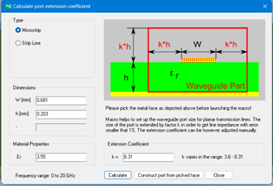
\includegraphics[width=0.55\linewidth]{Figures/chp2_CST_coefficient_calculator.png}
    \caption{Port extension coefficient macro in CST.}
    \label{fig:chp2_CST_coefficient_calculator}
    \end{figure}

As for the parameter sweeps, CST automatically lists all the versions together and if the parameter sweep was cancelled before it was completed, all the completed runs can still be viewed in the same manner.

    \begin{figure}[H]
    \centering
    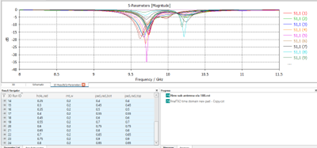
\includegraphics[width=0.85\linewidth]{Figures/chp2_CST_parameter_sweep.png}
    \caption{Parameter sweep in CST.}
    \label{fig:chp2_CST_parameter_sweep}
    \end{figure}

In industry FEKO is used for Farfield simulations such as antennas and CST is preferred for nearfield simulations such as X-Band vias and transitions. Keep in mind they are both capable of solving both nearfield and Farfield designs .

\section{ESA}
For a radar to measure the angle of a target more than one antenna is required, since the delay (\(\Delta d_{2}\)) is used to determine the angle (\(\theta\)) of the target. The delay (\(\Delta d_{2}\))) is measured as a phase delay and the phase can be converted to an angle of arrival using trigonometry. 

    \begin{figure}[H]
    \centering
    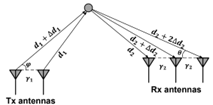
\includegraphics[width=0.4\linewidth]{Figures/chp2_angle_extraction.png}
    \caption{Angle extraction setup.}
    \label{fig:chp2_angle_extraction}
    \end{figure}

For the Tx antennas, a phase difference can be induced for each antenna which will then steer the main lobe in some direction (\(\Phi\)). This is known as beam steering. Beam steering is commonly used in Electronically Steered Arrays (ESA). These ESA typically consist of over 1000 individual antenna elements such as the AN/APG-63(V)1 radar with 1500 antenna elements \cite{reflectarrayy}.

\subsection{ESA Feeds}
Each antenna element for ESA requires a feed. These feeds usually include some gain control and a phase shifter. Four main types of feed networks exist namely Series, Parallel, Space-Fed and Reflective Space-Fed \cite{ESAfeed}. 

    \begin{figure}[H]
    \centering
    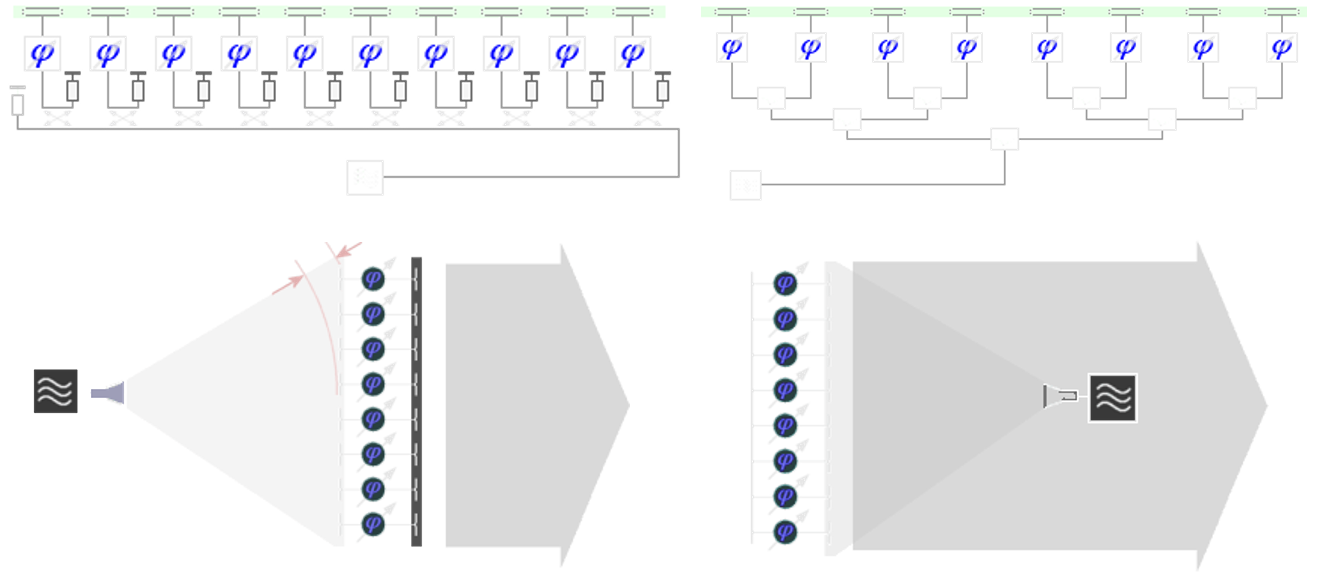
\includegraphics[width=0.8\linewidth]{Figures/chp2_ESA_feeds.png}
    \caption{Four types of ESA feeds.}
    \label{fig:chp2_ESA_feeds}
    \end{figure}

\section{Permittivity and Permeability}
A material’s electrical and magnetic characteristics can be partially defined by its permittivity and permeability. Permittivity is the ability of a material to store electrical potential energy under the influence of an electric field measured by the ratio of the capacitance of a capacitor with the material as dielectric to its capacitance with vacuum as dielectric \cite{Permittivty}. Permeability is the property of a magnetizable substance that determines the degree in which it modifies the magnetic flux in the region occupied by it in a magnetic field \cite{Permeability}. 

\section{VNA}
A Vector Network Analyzer uses advanced electronics and signal processing to analyse the system connected to the available ports. A VNA sends test signals sweeping through frequencies and measures the results at the available ports. The results are typically recorded as scattering parameters. A 2-port VNA will return a scattering matrix as shown below \cite{Sparams}. 
    \[\begin{bmatrix}
    S_{11} &  S_{12}\\
    S_{21} & S_{22}
    \end{bmatrix}\]

    \begin{figure}[H]
    \centering
    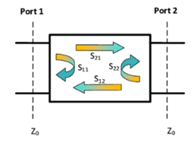
\includegraphics[width=0.4\linewidth]{Figures/chp2_Sparameters.png}
    \caption{Scattering parameters diagram.}
    \label{fig:chp2_Sparameters}
    \end{figure}

The subscripts refer to the port which received the signal and the port from which the signal is sent. Thus, the S11 parameter is the reflection coefficient for port 1. For a radar system the S21 parameter is import since it is the result at port 2 for a signal sent from port 1.




% ----------------------------------------------------
\ifstandalone
\bibliography{../Bibliography/References.bib}
\printnoidxglossary[type=\acronymtype,nonumberlist]
\fi
%\end{document}
% ----------------------------------------------------